\documentclass[12pt,letterpaper]{article}
\usepackage[utf8]{inputenc}
\usepackage[spanish]{babel}
\usepackage{amsmath}
\usepackage{amsfonts}
\usepackage{amssymb}
\usepackage{graphicx}
\usepackage{listings}
\usepackage{url}
\title{Tarea 5 \\ Optimizacion de Flujo de Redes}
\author{L.\ A.\ Gutierrez}

\usepackage{anysize} 
\marginsize{1.5cm}{1.5cm}{2.5cm}{2.5cm} 

\begin{document}

\maketitle


\section*{Introducción}
En esta practica se utilizó el concepto de distancia Manhattan\cite{Manhattan} para crear grafos de parecidos a cuadriculas, utilizamos el algoritmo Ford-Fulkerson\cite{Ford-Fulkerson} para medir el flujo entre el nodo inicial, el cual estaba definido como el primer nodo en la posición $(1,1)$ y el nodo final, el cual era el que se encontraba en la posición $(k,k)$, siendo $k$ la cantidad de filas y columnas del grafo ya que se realizo un grafo cuadrado. 


\section*{Distancia Manhattan}
La geometría del taxista, es una forma de geometría en la que la métrica usual de la geometría euclidiana es reemplazada por una nueva métrica en la que la distancia entre dos puntos es la suma de las diferencias absolutas de sus coordenadas. La métrica del taxista, en inglés se denomina geometría Taxicab, también se conoce como distancia rectilínea, distancia de ciudad, distancia Manhattan, o longitud Manhattan, con las correspondientes variaciones en el nombre de la geometría. El último nombre alude al diseño en cuadrícula de la mayoría de las calles de la isla de Manhattan, lo que causa que el camino más corto que un auto puede tomar entre dos puntos de la ciudad tengan la misma distancia que dos puntos en la geometría del taxista.

\section*{Ford-Fulkerson}
El algoritmo de Ford-Fulkerson propone buscar caminos en los que se pueda aumentar el flujo, hasta que se alcance el flujo máximo. La idea es encontrar una ruta de penetración con un flujo positivo neto que una los nodos origen y destino. Su nombre viene dado por sus creadores, L. R. Ford, Jr. y D. R. Fulkerson.

\textbf{Pseudocódigo de Ford-Fulkerson}\cite{Ford-Fulkerson}
\begin{verbatim}
 Ford-Fulkerson(G,s,t) { 
    for (cada arista (u,v) de E) { 
        f[u,v]= 0; 
        f[v,u]= 0; 
    } 
    while (exista un camino p desde s a t en la red residual Gf) { 
        cf(p) = min{cf(u,v): (u,v) está sobre p};
        for (cada arista (u,v) en p) { 
            f[u,v]= f[u,v] + cf(p); 
            f[v,u]= - f[u,v]; 
        }  
    } 
 }
\end{verbatim}

\section*{Método}
La actividad consistió en crear el grafo, con las siguientes restricciones:
\begin{itemize}
 \item $k$ es un parámetro entero el cual representara la cantidad de filas y columnas ya que es un cuadrado
 \item $P$ es un valor entre 0 y 1 el cual se obtiene de una probabilidad exponencial aleatoria.
 \item $l$ es la cantidad de conexiones que tendrá cualquier nodo con probabilidad $P$ de conectarse a otro nodo lejano, $l$ no puede ser mayor que $k$.
\end{itemize}
Se calculó el flujo máximo del grafo con el algoritmo Ford-Fulkerson, después realizamos la percolación\cite{Percolacion} de vértices y aristas, es decir, vamos eliminando vértices y aristas de forma aleatoria, y revisando el flujo máximo del grafo con el algoritmo Ford-Fulkerson.

\begin{figure}[htbp]
\centering
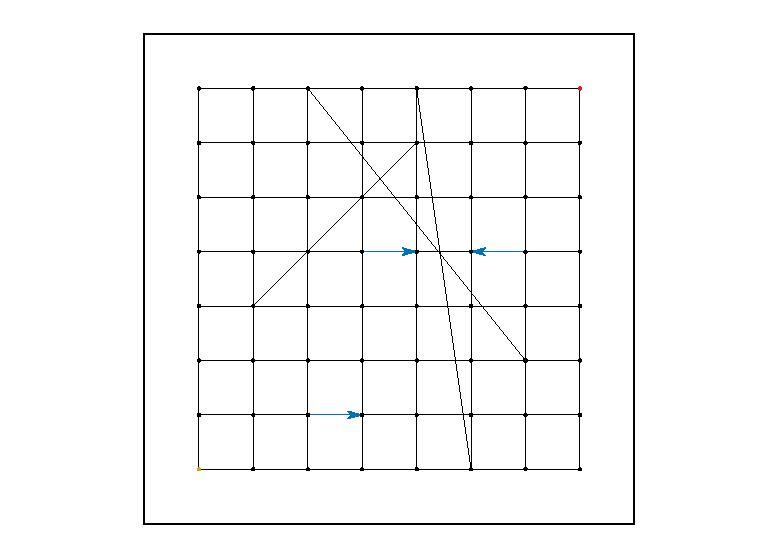
\includegraphics[scale=0.5]{NoPercola}
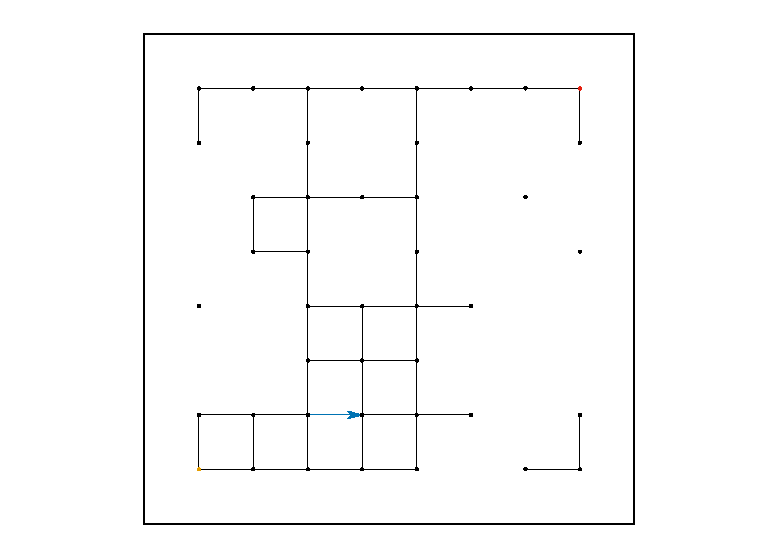
\includegraphics[scale=0.5]{PercolaNodo}
\caption{A la izquierda se representa un grafo con valor $k=8$, a la derecha el mismo grafo despues de realizar la percolación}
\end{figure}



\section*{Resultados}
El tiempo de ejecución de los grafos crece rápidamente con solo agregar una fila y columna, en este caso ejecuté instancias de valor $k=5$ hasta $k=20$ y al gratificarlos podemos ver el crecimiento.

\begin{figure}[htbp]
\centering
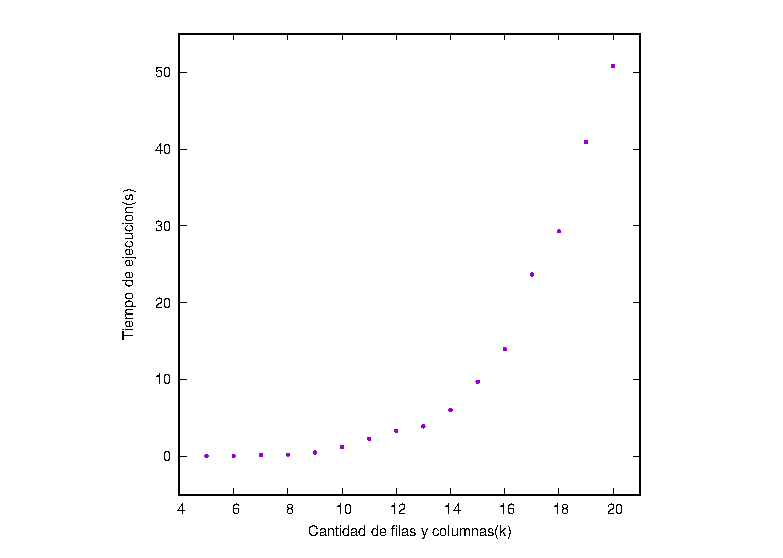
\includegraphics[scale=1]{Resultados}
\caption{Muestra la relación entre el tiempo de ejecución y el valor de $k$}
\end{figure}

\begin{thebibliography}{a}
\bibitem{Manhattan} \textit{Distancia Manhattan} \url{https://es.wikipedia.org/wiki/Geometr%C3%ADa_del_taxista}
\bibitem{Ford-Fulkerson} \textit{Algoritmo Ford-Fulkerson} \url{https://es.wikipedia.org/wiki/Algoritmo_de_Ford-Fulkerson}
\bibitem{Percolacion} \textit{Percolación} \url{http://dle.rae.es/?id=SXnI0kj}
\end{thebibliography}

\end{document}